\begin{figure}[ht]
    \centering
    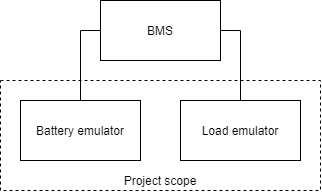
\includegraphics[scale=0.7]{System_context_diagram.png}
    \caption{System context diagram}
    \label{fig:system_context_diagram}
\end{figure}

The goal of this project is to design, built and test a battery pack emulator and (optionally) a load emulator that can be used to test a BMS (see figure \ref{fig:system_context_diagram}). This battery pack emulator should in the first design iteration be capable of emulating a battery pack with Li-ion cell characteristics. In order to emulate a Li-ion cell correctly it should be possible to emulate both charging and discharging of the Li-ion cell. 

Because the project team members are not yet experts in the field of designing battery pack emulators for BMS testing, it is chosen to design the battery pack emulator in iterations. In the first design iteration a battery pack emulator circuit will be designed which emulates the characteristics of a Li-ion battery pack. This battery pack emulator consists of two Li-ion cell emulators which are capable of charging and discharging. The voltages of each emulated cell are adjusted by a mechanical variable resistor. Each emulated cell has a voltage and current range that is 20\% larger than the safe operating area of a Li-ion cell.

In the second design iteration software will be added to the battery emulator circuit to control the voltages of each emulated cell via software. Also the temperature will be emulated in the battery pack emulator. The third design iteration consists of expanding the amount of emulated cells in the emulated battery pack to 14 cells. In the fourth design iteration a load emulator will be designed to test the BMS under different load conditions. This load emulator is capable of emulating electronics and motors. 

% The goal of this project is to design a programmable hardware system that presents a BMS with a "battery" and a "load" (see figure \ref{fig:system_context_diagram}). The hardware system emulates the battery and load. By using only software changes the hardware system should be able to emulate a battery with a different chemistry, capacity and cell topology. Likewise the hardware system should be able to emulate different loads from electronics through to motors under varying load.

At the end of the project it is expected that a battery pack emulator and optionally a load emulator is delivered. And if the planning allows it, a research report on existing battery and load emulators and the requirements for future battery and load emulators is delivered.

\section{Research questions}
In order to acquire functional requirements the following research questions have been derived:
% To be able to accomplish these deliverables the following research questions have been derived:
\begin{itemize}
    \item What is the safe operating area for Li-ion cells?
    % \item What different battery chemistries are there?
    % \item How do different battery chemistries behave?
    % \item What different battery cell topologies are there?
    % \item How do different battery cell topologies behave?
    % \item How do different battery capacities behave?
    % \item What kind of loads are there?
    % \item How do different loads behave?
    % \item How to control the voltage, current and phase to emulate a battery cell via software changes?
    % \item How to control the voltage, current and phase to emulate a load via software changes?
    \item How do existing battery emulators work?
    \item How do existing load emulators work?
    % \item What are the requirements for future emulators?
\end{itemize}

\section{Requirements}
For this project the following non-functional requirements with their functional requirements have been specified.

\begin{longtable}{|l|p{2in}|p{0.8in}|l|p{2in}|}
    \hline
    NF ID               & Non-functional                                                                                                                        & Design iteration            & F ID & Functional                                                                                                \\ \hline
    \multirow{3}{*}{1}  & \multirow{3}{*}{Battery pack emulator is able to emulate Li-ion characteristics}                                                      & \multirow{3}{*}{1}          & 1.1  & The maximum voltage of the battery pack emulator is 80V                                                   \\ \cline{4-5} 
                        &                                                                                                                                       &                             & 1.2  & The battery pack emulator has a peak power of 13.44kW (see 10.1)                                          \\ \cline{4-5} 
                        &                                                                                                                                       &                             & 1.3  & The battery pack emulator has a continuous power of 112W (see 10.1)                                       \\ \hline
    2                   & Battery pack emulator consists of two emulated Li-ion cells                                                                           & 1                           & 2.1  & The first iteration of the battery pack emulator consists of two  emulated Li-ion cells                   \\ \hline
    \multirow{3}{*}{3}  & \multirow{3}{*}{Battery pack emulator is able to emulate charging and discharging of Li-ion cell}                                     & \multirow{3}{*}{1}          & 3.1  & The emulated cell is able to deliver current (see 5.2 and 5.3)                                            \\ \cline{4-5} 
                        &                                                                                                                                       &                             & 3.2  & The emulated cell is able to sink current (see 5.4 and 5.5)                                               \\ \cline{4-5} 
                        &                                                                                                                                       &                             & 3.3  & A linear regulator is used to generate the specified voltages (see 5.1)                                   \\ \hline
    4                   & The voltages of each emulated cell can be adjusted separately via hardware                                                            & 1                           & 4.1  & The cell voltages can be changed by a mechanical variable resistor                                        \\ \hline
    \multirow{7}{*}{5}  & \multirow{7}{*}{Each emulated cell has a voltage and current range that is 20\% larger than the safe operating area of a Li-ion cell} & \multirow{7}{*}{1}          & 5.1  & The emulated cell has a voltage range of 2.48 to 5.04 V                                                   \\ \cline{4-5} 
                        &                                                                                                                                       &                             & 5.2  & The emulated cell has a peak sourcing current of 12A                                                      \\ \cline{4-5} 
                        &                                                                                                                                       &                             & 5.3  & The emulated cell has a continuous sourcing current of 100mA                                              \\ \cline{4-5} 
                        &                                                                                                                                       &                             & 5.4  & The emulated cell has a peak sinking current of 12A                                                       \\ \cline{4-5} 
                        &                                                                                                                                       &                             & 5.5  & The emulated cell has a continuous sinking current of 100mA                                               \\ \cline{4-5} 
                        &                                                                                                                                       &                             & 5.6  & The emulated cell has a peak power of 60W                                                                 \\ \cline{4-5} 
                        &                                                                                                                                       &                             & 5.7  & The emulated cell has a continuous power of 0.5W                                                          \\ \hline
    \multirow{3}{*}{6}  & \multirow{3}{*}{The voltages of each emulated cell can be adjusted separately via software}                                           & \multirow{3}{*}{2}          & 6.1  & The battery emulator hardware uses a microcontroller                                                      \\ \cline{4-5} 
                        &                                                                                                                                       &                             & 6.2  & A user interface is made to adjust the voltages                                                           \\ \cline{4-5} 
                        &                                                                                                                                       &                             & 6.3  & The voltages are adjusted using a digital potentiometer                                                   \\ \hline
    \multirow{3}{*}{7}  & \multirow{3}{*}{The battery pack emulator is able to emulate the temperature of the battery pack}                                     & \multirow{3}{*}{2}          & 7.1  & The temperature is emulated by using a digital potentiometer                                              \\ \cline{4-5} 
                        &                                                                                                                                       &                             & 7.2  & The emulated temperature range is -40 to 80 C                                                             \\ \cline{4-5} 
                        &                                                                                                                                       &                             & 7.3  & The emulated battery pack has an output which indicates the temperature relative to the output voltage    \\ \hline
    8                   & Battery pack emulator consists of 14 emulated Li-ion cells                                                                            & 3                           & 8.1  & 14 Li-ion cell emulators are wired in series                                                              \\ \hline
    \multirow{3}{*}{9}  & \multirow{3}{*}{The load emulator is capable of emulating electronics and motors}                                                     & \multirow{3}{*}{4}          & 9.1  & The load emulator is able to handle the battery pack voltage specified in 1.1                             \\ \cline{4-5} 
                        &                                                                                                                                       &                             & 9.2  & The load emulator is able to handle the battery pack power specified in 1.2                               \\ \cline{4-5} 
                        &                                                                                                                                       &                             & 9.3  & The load emulator can draw a current following a setpoint voltage which is generated by a microcontroller \\ \hline
    \multirow{3}{*}{10} & \multirow{3}{*}{The battery pack emulator and load emulator are safe}                                                                 & \multirow{3}{*}{1, 2, 3, 4} & 10.1 & The temperature of the electronics should be less than 25 C                                               \\ \cline{4-5} 
                        &                                                                                                                                       &                             & 10.2 & The input of the battery pack emulator has reverse polarity protection                                    \\ \cline{4-5} 
                        &                                                                                                                                       &                             & 10.3 & The input of the battery pack emulator and load emulator have over current protection                     \\ \hline
\end{longtable}

% \begin{longtable}{|c|p{10cm}|c|c|}
%     \hline
%     \textbf{ID} & \textbf{Requirement} & \textbf{Priority} & \textbf{Status}\\ \hline 
%     \textbf{U1} & The hardware is able to emulate a battery with a specific lithium-ion chemistry and capacity & Must & Proposed\\ \hline
%     \textbf{U2} & The hardware is flexible enough to require only software changes to emulate a battery with a different chemistry, a different capacity, and a different cell topology & Must & Proposed\\ \hline
%     % \textbf{U3} & The hardware is able to emulate different loads: from electronics through to motors under varying load & Must & Proposed\\ \hline
%     \textbf{U3} & The hardware system is able to adjust the load impedance characteristic curve & Must & Proposed\\ \hline
%     % \textbf{U4} & The hardware system is tested & Must & Proposed\\ \hline
%     \textbf{U4} & The hardware is able to control the voltage, current and phase independently & Must & Proposed\\ \hline
%     \textbf{U5} & The hardware contains a BMS & Won't & Proposed\\ \hline
% \end{longtable}



